% Preamble
\documentclass{article}


% Packages
\usepackage[legalpaper, portrati, margin=0.9in]{geometry}
\usepackage{amsmath}
\usepackage{bm}
\usepackage{amssymb}
\usepackage{gensymb}
\usepackage{mathtools}
\usepackage{xcolor}
\usepackage{caption}
\usepackage{subcaption}
\usepackage{pgfplots}
\pgfplotsset{compat=1.17}
\usepackage{tikz}
\usepackage{tkz-euclide}


% Macros
% @TODO: Figure out how to make \begin{center} and \begin[tabular} paired delimiters
\DeclarePairedDelimiter\ceil{\lceil}{\rceil}
\DeclarePairedDelimiter\floor{\lfloor}{\rfloor}

\newcommand*{\longunderscore}
{
\rule{0.25cm}{0.15mm}
}

% File info
\title{Algebra Notes}
\author{Eric Xia}
\date{Last Updated 21 August 2020}

% Document
\begin{document}

    \maketitle
    \tableofcontents
    \pagebreak

%%%-------------------------------------------NEW SECTION--------------------------------------%%%


    \section{Linear Functions}
    Linear equations involve an independent variable with degree 1. \\
    Forms of Linear Equations: \\

    %Table of the three linear function forms
    \begin{center}
        \begin{tabular}{|c|c|c|}
            \hline
            $y=mx+b$    & \textbf{Slope-Intercept} & $m$ is slope, $b$ is $y$-intercept \\
            \hline
            $y-y_1=m(x-x_1)$ & \textbf{Point-Slope} & $m$ is slope, $(x_1, y_1)$ is a point
            on the line \\
            \hline
            $Ax+By+C=0$ & \textbf{Standard}        & $A,B,C$ are integers and $A>0$     \\
            \hline
        \end{tabular}
    \end{center}

    \noindent The slope between two points $(x_1,y_1)$ and $(x_2,y_2)$ is given by
    $m=\frac{y_2-y_1}{x_2-x_1}$.

    \pagebreak
%%%-------------------------------------------NEW SECTION--------------------------------------%%%


    \section{Quadratic Functions}

    \subsection{Miscellaneous Quadratic Info}

    %Table with three forms of quadratic function
    \begin{center}
        \begin{tabular}{|c|c|}
            \hline
            $ax^2+bx+c$   & Standard Form  \\
            \hline
            $a(x-h)^2+k$  & Vertex Form    \\
            \hline
            $a(x-p)(x-q)$ & Intercept Form \\
            \hline
        \end{tabular}
    \end{center}

    \noindent The vertex is given by $(h,k)$, where $h=-\frac{b}{2a}$. The roots are given
    by $p$ and $q$. The intercept form is also known as the factored form. The
    \textbf{axis of symmetry} which divides a quadratic graph into right and left sides,
    is given by the line $x=-\frac{b}{2a}$.

    \subsection{Graphing Quadratic Functions}

    1. Find the vertex \\
    2. Find the $y$-intercept \\
    3. Find the $x$-intercept(s) \\
    4. Test two points minimum, one on each side of the vertex. \\
    5. Connect the points.

    % Graph of quadratic parent function
    \begin{center}
        \begin{tikzpicture}
            \begin{axis} [
            axis lines = center,
            xlabel = {$x$},
            ylabel = {$y$},
            xmajorticks=false,
            ymajorticks=false
            ]
                %%%
                \addplot [
                domain = -20:20,
                samples = 40,
                color = red
                ]
                {x^2};
                \addlegendentry{$y=x^2$}
            \end{axis}
        \end{tikzpicture}
    \end{center}

    \subsection{Factorization}

    \textbf{The Four Common Methods of Factoring:} \\
    \color{purple} \textbf{1. Greatest Common Factor} \color{black} \\
    $a(b+c)=ab+ac$ \\
    \color{purple} \textbf{2. Grouping} \color{black} \\
    This method is typically done with a four-term polynomial. Group the first two terms
    and the last two terms, then factor out a GCF from the two groups, and combine like
    polynomials. When the polynomial only has three terms, we can manipulate it so that the
    polynomial gains another term. We do this by multiplying the general quadratic
    coefficients $a$ and $c$ and then finding two factors of $ac$ which have a sum equal to
    the middle term's general coefficient, $b$. \\

    \noindent \color{blue} \textit{Example 1: Factor $x^3+7x^2+2x+14$} \color{black} \\
    \begin{align*}
        x^3+7x^2+2x+14 &= (x^3+7x^2) + (2x+14) \\
        &= (x^2(x+7) + 2(x+7)) \\
        &= (x+7)(x^2+2)
    \end{align*}

    \noindent \color{blue} \textit{Example 2: Factor $x^5-3x^3-2x^2+6$} \color{black} \\
    \begin{align*}
        x^5-3x^3-2x^2+6 &= (x^5-3x^3) - (2x^2-6) \\
        &= x^3(x^2-3) - 2(x^2-3) \\
        &= (x^2-3)(x^3-2)
    \end{align*}

    \noindent \color{blue} \textit{Example 3: Factor $3x^2+2x-8$} \color{black} \\
    The product $ac$ is given by $(3)(-8) = -24$. Its factors -4 and 6 have a sum of 2
    which is equal to $b$, the coefficient of the middle term. Thus, we can split the $2x$
    into two terms as below.

    \begin{align*}
        3x^2+\color{blue}2x\color{black}-8 &= 3x^2\color{blue}-4x+6x\color{black}-8 \\
        &= (3x^2-4x) + (6x-8) \\
        &= x(3x-4) + 2(3x-4) \\
        &= (3x-4)(x+2)
    \end{align*}

    \pagebreak
    \noindent \color{blue} \textit{Example 4: Factor $4x^2+10x-6$} \color{black} \\
    Again, the product $ac$ is given by $(4)(-6) = -24$. Its factors -2 and 12 have a sum
    of $b=10$. Thus, it can be factored by grouping:

    \begin{align*}
        4x^2+\color{blue}10x\color{black}-6 &= 4x^2\color{blue}-2x+12x\color{black}-6 \\
        &= (4x^2-2x) + (12x-6) \\
        &= 2x(2x-1) + 6(2x-1) \\
        &= (2x+6)(2x-1)
    \end{align*}

    \noindent \color{purple} \textbf{Special Forms:} \color{black} \\
    For factoring higher-degree polynomials, simply employ the usual methods of
    factorization. Below are some general factorizations that should be memorized.

    %Sum/Difference of Squares and Cubes
    \begin{center}
        \begin{tabular}{|c|c|}
            \hline
            $(a\pm b)^2 = a^2\pm 2ab+b^2$         & \textbf{Sum/Difference of Perfect Squares} \\
            \hline
            $a^2-b^2=(a+b)(a-b)$                  & \textbf{Difference of Squares}             \\
            \hline
            $a^3\pm b^3=(a\pm b)(a^2 \mp ab+b^2)$ & \textbf{Sum/Difference of Cubes}           \\
            \hline
        \end{tabular}
    \end{center}

    \subsection{Completing the Square}

    Taking a quadratic equation of the form $ax^2+bx+c=0$, completing the square allows us to
    rewrite this equation as $a(x+d)^2+e=0$, where $d=\frac{b}{2a}$ and $e=c-\frac{b^2}{4a}$.
    This method was inspired by the geometric representation of $x^2+bx$ being completed by
    $\left(\frac{b}{2}\right)^2$.

    \begin{figure} [hbt!]
        \centering
        \includegraphics [scale = 0.4] {Resources/Unit2Quadratics/Completing_The_Square.png}
    \end{figure}

    \noindent \color{blue} \textit{Example: Complete the square for $x^2+4x+1$} \color{black} \\
    $\left(\frac{b}{2}\right)^2 = 4$, so we add 4 and subtract 4. Parantheses are added to
    better conceptualize the later simplification.

    \begin{align*}
        (x^2+4x+4)+1-4 &= (x^2+4x+4) - 3 \\
        &= (x+2)^2 - 3
    \end{align*}

    \subsection{The Loh Method}

    Originally devised by ancient Babylonians and Greeks, this method was revised by Viete
    and rediscovered by Professor Po-Shen Loh in late 2019. We will refer to this as the
    Loh Method for ease of explanation. \\

    \noindent \color{blue} \textit{Example 1: Solve $x^2-14x+24=0$} \color{black} \\
    The factorization will be in the form $(x-\longunderscore)(x-\longunderscore)$.
    The method says that \textit{if and only if} we can find two numbers such that their sum
    is the opposite of $b$, in this case 14, and their product is $c$ which is 24 in this case
    then those numbers are the solutions. This method is an extremely convenient way of finding
    the solutions for \textit{any} quadratic equation, even irrational ones that would be hard
    to guess. \\

    \noindent This method uses the concept that our two numbers that add to 14 have an average
    of 7, since $\frac{14}{2} = 7$. Taking the average of two numbers, we know that one of the
    factors will be a little smaller than 7 and the other factor will be a little greater than
    7. We can express the smaller factor by "7-$u$" and the greater factor by "7+$u$". We know
    that the factors have a product of 24, thus

    \begin{align*}
        24  &= (7-u)(7+u) \\
        &= 49 - u^2 \\
        u^2 &= 25 \\
        u   &= \pm 5
    \end{align*}

    \noindent Since $u = \pm 5$ exists, we can calculate $7-u = 7-5 = 2$ and $7+u=7+5=12$.
    Using $u=-5$ would produce the same values. Now we plug 2 and 12 into
    $(x-\longunderscore)(x-\longunderscore)$, giving us

    \begin{align*}
        0          &= x^2-14x+24 \\
        &= (x-2)(x-12) \\
        \implies x &= 2,12
    \end{align*}

    \noindent Using other factorization methods, we verify that these are indeed the solutions
    to the quadratic equation. \\

    \noindent \color{blue} \textit{Example 2: Solve $x^2-8x+13=0$} \color{black} \\
    Using other methods, we would not have been able to factor this since 13 is a prime number.
    Again, $x^2-8x+13 = 0 = (x-\longunderscore)(x-\longunderscore)$. \\

    \noindent If we can find two numbers that have a sum of 8 and a product of 13, then they
    are the solutions. Looking at the product which is 13, it's very hard to think of factors
    of 13 which have a sum of 8. Once again, there are two numbers that have an average of 8,
    so we will need $u$ to satisfy the below equation.

    \begin{align*}
        13  &= (4-u)(4+u) \\
        &= 16 - u^2 \\
        u^2 &= 3 \\
        u   &= \pm \sqrt{3}
    \end{align*}

    \noindent We can ignore the negative value of $u$ since it will give the same values as its
    opposite. Thus, \\

    \begin{align*}
        0          &= x^2-8x+13 \\
        &= \left(x-[4-\sqrt{3}]\right) \left(x-[4+\sqrt{3}]\right) \\
        \implies x &= 4 \pm \sqrt{3}
    \end{align*}

    \subsection{The Quadratic Formula}

    We can derive the quadratic formula through completing the square. \\

    \begin{align*}
        ax^2+bx+c                                                                 &=  0 \\
        (ax^2+bx)+c                                                               &=  0 \\
        a\left(x^2+x\cdot\frac{b}{a}\right)+c                                     &= 0 \\
        a\left(x^2+x\cdot\frac{b}{a}+\frac{b^2}{4a^2}\right)+c-\frac{b^2}{4a^2}   &= 0 \\
        a\left(x^2+x\cdot\frac{b}{a}+\frac{b^2}{4a^2}\right)+c = \frac{b^2}{4a^2} &= \frac{b^2}{4a^2} \\
        a\left(x+\frac{b}{2a}\right)^2   &= \frac{b^2}{4a} - c \\
        \left(x+\frac{b}{2a}\right)^2   &= \frac{b^2}{4a^2} - \frac{c}{a} \\
        \left(x+\frac{b}{2a}\right)^2   &= \frac{b^2-4ac}{4a^2} \\
        x + \frac{b}{2a}                &= \pm\frac{\sqrt{b^2-4ac}}{2a}
    \end{align*}

    \begin{equation*}
        \bm{{x &= \frac{-b\pm\sqrt{b^2-4ac}}{2a}}}
    \end{equation*}

    \subsection{Imaginary and Complex Numbers}

    When a quadratic solution involves a negative number under a radicand, that solution is
    either imaginary or complex. Recall that pure imaginary numbers are of the form $bi$,
    where $i=\sqrt{-1}$ and complex numbers are of the form $a+bi$. \\

    \noindent \color{blue} \textit{Example 1: $x^2+4x+5=0$} \color{black} \\
    Using the quadratic formula, we compute $x$ to be \\

    \begin{align*}
        x &= \frac{-4\pm\sqrt{-4}}{2} \\
        &= \frac{-4\pm 2i}{2} \\
        &= -2 \pm i
    \end{align*}

    \noindent If we wanted to efficiently find the behavior of a quadratic's roots, we could use the
    \textbf{discriminant}, $b^2-4ac$. \\

    % Table describing relationship between discriminant and roots
    \begin{center}
        \color{purple} \textbf{Types of Roots} \color{black} \\
        %%%
        \begin{tabular}{|c|c|c|}
            \hline
            Discriminant is positive & Discriminant is zero   & Discriminant is negative   \\
            \hline
            $b^2-4ac>0$              & $b^2-4a=0$             & $b^2-4ac<0$                \\
            \hline
            \textit{Two Real Roots}  & \textit{One Real Root} & \textit{Two Complex Roots} \\
            \hline
        \end{tabular}
    \end{center}

    \subsection{Mathematical Modeling with Quadratic Functions}

    Quadratic functions are often used for modeling flying objects, for example the flight trajectory of a thrown
    ball. Consider the graph of $f(t) = -(t-3)^2+9$, where $t>0$. If $t$ represents time, then
    $f(t)$ represents the height at which the ball is at a particular time. We can then clearly
    see from the graph that the ball is at a height of 0 when time is 0. The ball reaches its peak
    height of 9 at the vertex of the quadratic function when time is 3, and descends to a height of
    0 at the second root of the function.

    \begin{center}
        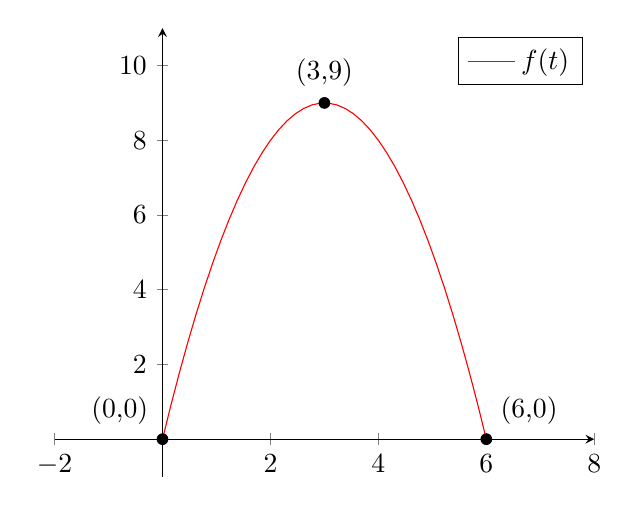
\begin{tikzpicture}
            \begin{axis} [
            axis lines = center,
            ymin = -1,
            ymax = 11,
            xmin = -2,
            xmax = 8
            ]
                %%%
                \addplot [
                domain = 0:6,
                samples = 40,
                color = red
                ]
                {-(x-3)^2+9};
                \addlegendentry{$f(t)$}
                %%%
                \node[label={135:{(0,0)}},circle,fill,inner sep=1.5pt] at (axis cs:0,0) {};
                \node[label={90:{(3,9)}},circle,fill,inner sep=1.5pt] at (axis cs:3,9) {};
                \node[label={45:{(6,0)}},circle,fill,inner sep=1.5pt] at (axis cs:6,0) {};
            \end{axis}
        \end{tikzpicture}
    \end{center}

    \pagebreak
%%%-------------------------------------------NEW SECTION--------------------------------------%%%


    \section{Polynomials}

    \subsection{Long Division}

    \color{purple} \textbf{Dividend = Divisor $\cdot$ Quotient + Remainder} \color{black} \\
    \noindent $f(x)=d(x)\cdot q(x)+r(x)$ \\
    \noindent Note that the degree of $r(x)$ is always less than that of $d(x)$. \\

    \noindent \color{blue} \textit{Example 1: Divide $2x^2-5x-1$ by $x-3$} \color{black} \\

    \begin{figure} [hbt!]
        \centering
        \includegraphics[scale = 0.8] {Resources/Unit3Polynomials/longdiv.PNG}
    \end{figure}

    \begin{equation*}
        \therefore 2x^2-5x-1 = (x-3)(2x+1)+2
    \end{equation*}

    \noindent where the remainder is 2. \\

    \noindent \color{purple} \textbf{The Remainder Theorem:} \color{black} \\
    \noindent When a polynomial $f(x)$ is divided by $x-c$ the remainder is $f(c)$. \\

    \noindent \color{blue} \textit{Example 2: Find the remainder when $2x^2-5x-1$ is
    divided by $x-5$} \color{black} \\

    \begin{align*}
        f(5) &= 2(5)^2-5(5)-1 \\
        &= 50-25-1 \\
        &= 24
    \end{align*}

    \noindent Thus, the remainder is 24. \\
    \noindent \color{purple} \textbf{The Factor Theorem:} \color{black} \\
    When $f(c)=0$, $x=c$ is a factor of $f(x)$. The converse of this is also true.

    \subsection{Synthetic Division}

    Synthetic division is a shortcut for long division. It only works when the divisor is
    of the first degree. The remainder produced by synthetic division is also the the value
    of the function at the remainder, $f(r)$ when $r$ is the remainder. \\

    \noindent \color{blue} \textit{Example: Divide $x^3-2x^2+3x-4$ by $x-2$} \color{black} \\

    \noindent 1. Draw a table like so and write $c$ on the left side of the table, for a
    divisor in the form $x-c$. In this case, $c=2$. \\

    \begin{figure} [hbt!]
        \centering
        \includegraphics [scale = 0.5] {Resources/Unit3Polynomials/synthdiv1.png}
    \end{figure}

    \noindent 2. Add the coefficients of the polynomial's terms under the line as is. In
    this case, the coefficients corresponding to $x^3, x^2, x^1,$ and $x^0$ are $1,-2,3,$
    and $-4$, respectively. \\

    \begin{figure} [hbt!]
        \centering
        \includegraphics [scale = 0.5] {Resources/Unit3Polynomials/synthdiv2.png}
    \end{figure}

    \noindent 3. Drop the first coefficient, in this case 1, below the newly made bar. Then
    write the product of $c$ and the first coefficient below the second coefficient. Now
    write the sum of the second coefficient and this product below the bar. \\

    \begin{figure} [hbt!]
        \centering
        \includegraphics [scale = 0.5] {Resources/Unit3Polynomials/synthdiv3.png}
    \end{figure}

    \noindent 4. Find the product of $c$ and the calculated sum, in this case the second
    green number. Find the sum of this product and the third coefficient. Repeat this
    process for the rest of the coefficients. The last calculated sum is the remainder,
    in this case the purple number.

    \begin{figure} [hbt!]
        \centering
        \includegraphics [scale = 0.5] {Resources/Unit3Polynomials/synthdiv4.png}
        \includegraphics [scale = 0.5] {Resources/Unit3Polynomials/synthdiv5.png}
    \end{figure}

    \noindent 5. The three green sums are the coefficients of the quotient. The quotient
    should be of degree 2, since its largest term $x^3$ divided by the divisor's largest
    term, $x$, is $x^2$. Thus, $x^2$ corresponds to the first green number, and so on.
    Here, $c$ refers to the constant term of the polynomial.

    \begin{figure} [hbt!]
        \centering
        \includegraphics [scale = 0.5] {Resources/Unit3Polynomials/synthdiv6.png}
    \end{figure}

    \noindent Thus,

    \begin{align*}
        \frac{x^3-2x^2+3x-4}{x-2} &= 1x^2+0x+3+\frac{2}{x-2} \\
        &= x^2+3+\frac{2}{x-2}
    \end{align*}

    \subsection{Vieta's Formulas}

    Vieta’s Formulas relate the coefficients of polynomials to the sums and products of their
    roots. Whereas Vieta’s Formulas seem trivial in quadratic applications, they become
    extremely useful in complex polynomials with many roots or roots that are hard to derive.
    Vieta’s Formulas can be viewed as a shortcut for finding solutions of a polynomial quickly
    simply through the sums and products of the roots. \\

    \noindent Consider the polynomial $x^2+2x-15=(x-3)(x+5) \implies x=-5,3$. Using Vieta's
    Formulas, we can find the sum of the roots $3+(-5)=-2$ and $3\cdot(-5)=-15$ directly,
    without having to find each root directly. \\

    \noindent By the Remainder Factor Theorem, a polynomial $f(x)$ has roots $r_1$ and $r_2$
    in the form $f(x)=A(x-r_1)(x-r_2)=Ax^2-A(r_1+r_2)x+Ar_1 r_2$ for some constant $A$.
    Comparing coefficients with $f(x) = ax^2+bx+c$, we can conclude that $a=A, b=-A(r_1+r_2)$,
    and $c=Ar_1 r_2$. Hence, we get: \\

    \noindent \color{purple} \textbf{Vieta's Formulas for Quadratics:} \color{black} \\
    \noindent Given $f(x) = ax^2+bx+c$ if the equation $f(x)=0$ has roots $r_1$ and $r_2$, then

    \begin{equation*}
        r_1 + r_2 = -\frac{b}{a}, r_1 r_2 = \frac{c}{a}
    \end{equation*}

    \noindent Alternatively,

    \begin{equation*}
        b=-(p+q),c=pq
    \end{equation*}

    \noindent It is important to note that the precondition for using Vieta's Formula is that
    the polynomial $f(x)$ must be put in a \textbf{monic} form, that is, the leading coefficient
    $a$ must be 1. \\

    \noindent \color{blue} \textit{Example 1: If $\alpha$ and $\Beta$ are the roots of the
    quadratic $x^2-4x+9=0$, what are the values of} \\
    \noindent 1. $\alpha+\Beta$ \\
    \noindent 2. $\alpha\Beta$ \\
    \noindent 3. $\alpha^2\Beta^2$ \color{black} \\

    \noindent 1.
    \begin{equation*}
        \alpha + \Beta = -\frac{b}{a} = -\frac{-4}{1} = 4
    \end{equation*}

    \noindent 2.
    \begin{equation*}
        \alpha\Beta = \frac{c}{a} = \frac{9}{1} = 9
    \end{equation*}

    \noindent 3.
    \begin{align*}
        \alpha^2+\Beta^2 &= (\alpha + \Beta)^2 - 2\alpha\Beta \\
        &= 4^2 - 2(9) \\
        &= -2
    \end{align*}

    \noindent For this question, the roots were $2\pm i\sqrt{5}$. vieta's Formulas offer a
    simpler approach to compute these expressions without potentially making calculation
    mistakes. \\

    \noindent \color{blue} \textit{Example 2: What are the roots of the quadratic $x^2-5x+6$?} \color{black} \\
    \noindent If $p$ and $q$ are the roots of the quadratic, then $p+q=5$ and $pq=6$. Solving
    this system, it's easy to see that the roots are 2 and 3. \\

    \noindent \color{blue} \textit{Example 3: Find a quadratic with roots 2 and 5.} \color{black} \\
    $b=-(2+5)=-7, c=(2)(5)=10$ \\
    Hence, the desired quadratic is $x^2-7x+10$.

    \pagebreak
    \noindent \color{blue} \textit{Example 4: Find a quadratic with roots $3+2i$ and $3-2i$.} \color{black} \\
    \noindent $b=-[(3+2i)+(3-2i)] = -6,c=(3+2i)(3-2i)=13$. \\
    \noindent The desired quadratic is $x^2-6x+13$.

    \noindent We can also generalize these formulas to higher-degree polynomials: \\
    \noindent \color{purple} \textbf{Vieta's Formula:} \color{black} \\
    Let $P(x)=a_n x^n + a_{n-1}x^{n-1}+\dots+a_0$ be a polynomial with complex coefficients
    and degree $n$, having complex roots $r_n, r_{n-1},\dots,r_1$. Then for any integer
    $0\leq k \leq n$, \\

    \begin{equation*}
        \sum\limits_{1\leq i_1 < i_2<\dots<i_k\leq n}   r_{i_1}r_{i_2}\dots r_{i_k}
        = (-1)^k \frac{a_{n-k}}{a_n}
    \end{equation*}

    \noindent Vieta's Formulas for quadratic polynomials written in summation notation is \\
    \begin{equation*}
        \sum\limits_{i=1}^n r_i     = -\frac{a_{n-1}}{a_n}, r_1r_2\dots r_n=(-1)^n\frac{a_0}{a_n}
    \end{equation*}

    \noindent \color{blue} \textit{Example 5: Suppose $k$ is a number such that the cubic
    polynomial $P(x)=-2x^3+48x^2+k$ has three integer roots that are all prime numbers. How
    many possible distinct values are there for $k$?} \color{black} \\

    \noindent Let $p,q,$ and $r$ denote the three integer roots of $P(x)$. Then by Vieta's
    Formula, we have $pq+qr+pr=0$ but since $p,q,r$ are prime, each of them are strictly
    greater than 1 and hence no such $P(x)$ exists.

    \pagebreak
%%%-------------------------------------------NEW SECTION--------------------------------------%%%


    \section{Higher-degree Polynomials}

    \subsection{Graphing Higher-degree Polynomials}
    \color{purple} \textbf{Steps to Graph Higher-Degree Polynomials:} \color{black} \\

    \noindent 1. Determine the zeroes of the polynomial $P(x)$ and their multiplicity. \\
    2. Determine the $y$-intercept, $(0, P(0))$ \\
    3. Use the Leading Coefficient Test to determine the end behaviors. \\
    4. Plot a few more points to make the sketch more accurate.
    At least plot one point at each end and between each of the zeroes. \\

    \noindent The first three names of higher-degree polynomials are \textbf{cubic} ($x^3$),
    quartic ($x^4$), and quintic ($x^5$). Polynomials that are second-degree and higher
    tend to be \textit{continuous} and there are usually local maxima and minima. \\

    \noindent A polynomial with degree $n$ will have at most $n-1$ extrema. \\

    \noindent \color{purple} \textbf{The Multiplicity Test}: \\

    \noindent \color{black}
    If $x=r$ is a zero of the polynomial $P(x)$ with multiplicity $k$ then:  \\
    1. If $k$ is odd then the $x$-intercept corresponding to $x=r$ will cross the x-axis. \\
    2. If $k$ is even then the $x$-intercept corresponding to $x=r$ will only touch the
    x-axis and not cross it. \\

    \noindent Furthermore, if $k>1$ then the graph will flatten out at $x=r$. \\

    \noindent \color{purple} \textbf{Multiplicity} \color{black} refers to the number of
    times a factor is found within a polynomial. Consider the polynomial given by
    $P(x)=x^2(x-3)(x+2)$. Its zeroes are $x=-2$ ($k=1$), $x=0$ ($k=2$), and
    $x=3$ ($k=1$). $x=0$ has a mutliplicity of 2, since the factor appears twice.
    Recall that $x^2=0$ gives $x=\pm 0$. \\


    \noindent \color{purple} \textbf{The Leading Coefficient Test:} \color{black} Suppose
    that $P(x)$ is a polynomial with degree $n$, where $P(x)=ax^n+\dots$. We only need to
    consider the first coefficient, $a$. \\

    \noindent 1. If \textbf{$a>0$ and $n$ is even} then the graph of $P(x)$ will increase without
    bound at both endpoints. \\
    \begin{figure} [hbt!]
        \centering
        \includegraphics[scale = 0.5] {Resources/Unit4HigherPolynomials/leadcoeff1.png}
    \end{figure}

    \noindent 2. If \textbf{$a>0$ and $n$ is odd} then the graph of $P(x)$ will increase without bound
    at the right end and decrease without bound at the left end. \\
    \begin{figure} [hbt!]
        \centering
        \includegraphics[scale = 0.5] {Resources/Unit4HigherPolynomials/leadcoeff2.png}
    \end{figure}

    \noindent 3. If \textbf{$a<0$ and $n$ is even} then the graph of $P(x)$ will decrease without
    bound on both ends. \\
    \begin{figure} [hbt!]
        \centering
        \includegraphics[scale = 0.5] {Resources/Unit4HigherPolynomials/leadcoeff3.png}
    \end{figure}

    \noindent 4. If \textbf{$a<0$ and $n$ is odd} then the graph of $P(x)$ will decrease without
    bound at the right end and increase without bound at the left end. \\
    \begin{figure} [hbt!]
        \centering
        \includegraphics[scale = 0.5] {Resources/Unit4HigherPolynomials/leadcoeff4.png}
    \end{figure}


    \noindent \color{blue} \textit{Example: Sketch the graph of $P(x)=x^4-x^3-6x^2$}. \color{black} \\
    $P(x)=x^2(x-3)(x+2)$ \\
    Multiplicity is 1 at $x=-2$ \\
    Multiplicity is 2 at $x=0$ \\
    Multiplicity is 1 at $x=3$ \\

    \noindent Thus, the zeroes at $x=-2$ and $x=3$ correspond to x-intercepts, whereas the
    zero at $x=0$ has an even multiplicity so it will only touch the x-axis instead of
    crossing it. The $y$-intercept is $(0,0)$ and this is also the $x$-intercept.
    Some function evaluations are below. \\
    \begin{center}
        \begin{tabular}{ccc}
            $P(-3)=54$ & $P(-1)=-4$ & $P(4)=96$
        \end{tabular}
    \end{center}

    \noindent The leading coefficient is 1 and the highest degree of $P(x)$ is 4 which is
    an even number so by the Leading Coefficient Test, both ends of the polynomial's graph
    will increase without bound. Putting all our information together, we can now sketch
    the graph. \\

    \begin{center}
        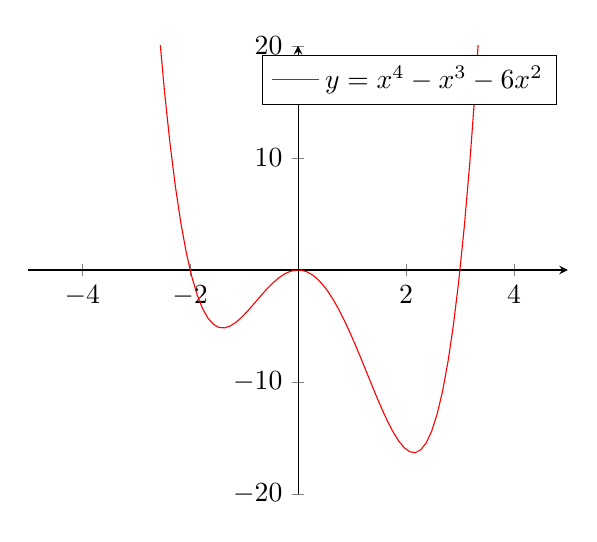
\begin{tikzpicture}
            \begin{axis}[
            axis lines = center,
            ymin = -20,
            ymax = 20,
            xmin = -5,
            xmax = 5
            ]
                \addplot [
                samples=100,
                color=red
                ]
                {x^4-x^3-6*x^2};
                \addlegendentry{$y=x^4-x^3-6x^2$}
            \end{axis}
        \end{tikzpicture}
    \end{center}

    \subsection{Rational Root Test}

    Suppose we have a polynomial $P(x)$ with integer coefficients and a nonzero constant
    term, $a_n\not=0$. \\
    $P(x)=a_nx^n+a_{n-1}x^{n-1}+\dots+a_1x+a_0$ \\
    Then potential rational roots of $P(x)$ are of the form

    \begin{equation*}
        \frac{p}{q} = \frac{\pm\text{factors of }a_0}{\pm\text{factors of }a_n}
    \end{equation*}

    \noindent \color{blue} \textit{Example: Find the rational roots of
    $P(x)=3x^3-4x^2-17x+6$} \color{black} \\

    \noindent The leading coefficient is $a_n=3$ and constant term is $a_0=6$.
    We can determine the positive and negative factors of \\
    $a_0=6:\pm(1,2,3,6)$ \\
    $a_n=3:\pm(1,3)$ \\
    Then \\

    \begin{equation*}
        \frac{p}{q} = \frac{\pm(1,2,3,6)}{\pm(1,3)} = \pm 1, \pm\frac{1}{3}, \pm 2,
        \pm \frac{2}{3}, \pm 3, \pm \frac{3}{3}, \pm \frac{6}{1}, \pm \frac{6}{3}
    \end{equation*}

    \noindent Eliminating duplicate terms and simplifying, our root candidates are:

    \begin{equation*}
        \pm \frac{1}{3}, \pm\frac{2}{3}, \pm 1, \pm 2, \pm 3, \pm 6
    \end{equation*}

    \noindent We recall that if $a$ is a root of $P(x)$ then $P(a)=0$. Let's check our
    candidates now.

    % Table of candidates and if they are roots of function
    \begin{center}
        \begin{tabular}{|c|c|}
            \hline
            \textbf{$P(x)=3x^3-4x^2-17x+6$} & \textbf{Is it a root?} \\
            \hline
            $P(\frac{1}{3})=0$              & YES                    \\
            \hline
            $P(-\frac{1}{3})=\frac{100}{9}$ & No                     \\
            \hline
            $P(\frac{2}{3}=-\frac{56}{9}$   & No                     \\
            \hline
            $P(-\frac{2}{3})=\frac{44}{3}$  & No                     \\
            \hline
            $P(1)=-12$                      & No                     \\
            \hline
            $P(-1)=16$                      & No                     \\
            \hline
            $P(2)=-20$                      & No                     \\
            \hline
            $P(-2)=0$                       & YES                    \\
            \hline
            $P(3)=0$                        & YES                    \\
            \hline
            $P(-3)=-60$                     & No                     \\
            \hline
            $P(6)=408$                      & No                     \\
            \hline
            $P(-6)=-684$                    & No                     \\
            \hline
        \end{tabular}
    \end{center}

%%%-------------------------------------------NEW SECTION--------------------------------------%%%


    \section{More Functions}

    \subsection{Composite Functions}
    Function composition refers to when one function is applied to the results of another.
    The formal notation of "the result of function $f$ sent through function $g$ is written
    $(g\circ f)(x)$ which is also the same as saying $g(f(x))$. \\

    \noindent \color{blue} \textit{Example: Given $f(x)=3x+2$ and $g(x)=x+5$,
    find $(f\circ g)(x)$}. \color{black} \\

    \begin{align*}
        (f\circ g)(x) &= f(x+5) \\
        &= 3(x+5)+2 \\
        &= 3x+17
    \end{align*}

    \subsection{Inverse Functions}
    An \textbf{inverse function} is a function that reverses another function. If a function
    $f(x)=y$ then its inverse, denoted by the superscript -1, is given by $f^{-1}(y)=x$.
    The inverse function is also commonly wrote as $g(x)$. \\

    \noindent An \textbf{invertible function} is a function that has an inverse. A function
    is invertible if and only if the function is \textbf{one-to-one}, or for each $y$-value,
    there must be only one value of $x$ such that $Y\rightarrow X$. Such a function is also
    described as \textbf{bijective}. A function is bijective only if and only if it passes the
    horizontal line test. Inverse functions are symmetrical across the line $y=x$. \\

    \noindent \color{blue} \textit{Example: Given $f(x)=\sqrt{x-3}$, find $g^{-1}(x)$ for
    $x\geq0$}. \color{black} \\

    \begin{align*}
        y=f(x) &= \sqrt{x-3} \\
        x &= \sqrt{y-3} \\
        x^2 &= y-3 \\
        x^2+3 &= y \\
        g^{-1}(x) &= x^2+3
    \end{align*}

    \pagebreak
%%%-------------------------------------------NEW SECTION--------------------------------------%%%


    \section{Exponents and Logarithms}

    \subsection{Review of Exponents and Logarithms}

    \color{purple} \textbf{Exponent Laws:} \color{black} \\
    1. $a^ma^n=a^{m+n}$ \\
    2. $(a^m)^n=a^{mn}$ \\
    3. $(ab)^m=a^mb^m$ \\
    4. $\frac{a^m}{a^n}=a^{m-n},a\not=0$ \\
    5. $(\frac{a}{b})^m=\frac{a^m}{b^m},b\not=0$ \\
    6. $a^-m=\frac{1}{a^m},a\not=0$ \\
    7. $a^{\frac{1}{n}}=\sqrt[n]{a}$ \\
    8. $a^0=1,a\not=0$ \\
    9. $a^{\frac{m}{n}}=\sqrt[n]{a^m}=(\sqrt[n]{a})^m$ \\

    \noindent Logarithms are the inverse operation of exponents. In other words, \\
    $y=\log_ax\iff x=a^y, a>0$ \\
    where $a$ is the base. Conventionally, if a base is unspecified then it is 10 such that
    $\log x = \log _{10} x$. \\

    \noindent The natural logarithm, $\ln{x}$, is a logarithm with base $e$. \\

    \noindent \color{purple} \textbf{Logarithm Properties:} \color{black} \\
    1. $\log _a xy=\log _a x+\log _a y$ \\
    2. $\log _a \frac{x}{y}=\log _a x - \log _a y$ \\
    3. $\log _a x^y=y\cdot\log _a x$ \\
    4. $\log _a a^x=x$ \\
    5. $a^{\log _a x} = x$ \\
    6. $\log _a \frac{1}{x}=-\log _a {x}$ \\

    \noindent \color{purple} \textbf{Common Logarithms:} \color{black} \\
    1. $\ln{e}=1$ \\
    2. $\log _a {1}=0, a>0$ \\
    3. $\log _a {0} = $ UND \\
    4. $\log _a {a} = 1, a>0$

    \subsection{Graphing Exponential and Logarithmic Functions}

    The function $y=e^x$ is the inverse of $y=\ln{x}$. From the graph, we can see that the
    two functions are symmetric across the line $y=x$. There is a horizontal asymptote at
    $y=0$ in the graph of $e^x$ and a vertical asymptote at $x=0$ in the graph of $y=\ln{x}$.

    \begin{center}
        \begin{tikzpicture}
            \begin{axis}[
            axis lines = center,
            xmin = -10,
            xmax = 10,
            ymin = -10,
            ymax = 10
            ]
                %y=ln(x)
                \addplot [
                domain=0:10,
                samples=100,
                color=red
                ]
                {ln(x)};
                \addlegendentry{$y=\ln{x}$}
                %y=e^x
                \addplot [
                domain=-5:10,
                samples=100,
                color=blue
                ]
                {e^x};
                \addlegendentry{$y=e^x$}
                %y=x
                \addplot[
                domain = -10:10,
                samples=100,
                color=black,
                style=dashed
                ]
                {x};
            \end{axis}
        \end{tikzpicture}
    \end{center}

    \pagebreak
%%%-------------------------------------------NEW SECTION--------------------------------------%%%


    \section{Radical Functions}

    Radical Functions are functions that contain a fractional exponent, that is, a variable
    under a radicand. When graphing radical functions, it is important to keep the domain in
    mind. For the parent function $f(x)=\sqrt{x}$, the domain is $x\geq 0$. This results from
    the fact that real solutions will not come from the square root of negative numbers. \\

    \noindent For the square root function $f(x)=a\sqrt{x}$, we notice that a value
    $|a|>0\implies$ a vertical stretch and $0<|a|<1\implies$ a vertical shrink. If $a<0$ then
    the graph will be vertically reflected across the $x$-axis. \\

    \noindent Radical functions are graphed by plotting many points while keeping in mind the
    domain and connecting them with a line.

    \pagebreak
%%%-------------------------------------------NEW SECTION--------------------------------------%%%


    \section{Rational Functions}

    A rational function is any function that can be expressed as the ratio of two polynomial
    functions, where the denominator is not equal to 0. The domain of a rational function
    $f(x)=\frac{P(x)}{Q(x)}$ is the set of all points for which $Q(x)\not=0$.
    \textbf{Singularities} are the $x$-values at which rational functions are undefined, for
    which $Q(x)\not=0$. \\

    \noindent \textbf{Oblique Asymptotes} are asymptotes that are neither perpendicular nor
    parallel, rather, they are inclined. Vertical asymptotes occur at all singularities for
    rational functions, and a rational function can have at most one horizontal/oblique asymptote. \\

    \noindent If a function $f(x)=\frac{P(x)}{Q(x)}$ has a highest degree of $n$ in the numerator
    and $m$ in the denominator then: \\

    % Table with asymptote types
    \begin{center}
        \begin{tabular}{|c|c|}
            \hline
            $n>m$ & No Horizontal Asymptote (Although if $n=m+1$ then there is an Oblique Asymptote)            \\
            \hline
            $n<m$ & $x$-axis is a Horizontal Asymptote                                                          \\
            \hline
            $n=m$ & Horizontal Asymptote exists at $y=\frac{\text{Coefficient of }        n}{\text{Coefficient of } m}$ \\
            \hline
        \end{tabular}
    \end{center}

    \noindent \color{blue} \textit{Example 1: Find any horizontal or oblique asymptotes for
    $f(x)=\frac{2x^2+x+1}{x^2+16}$} \color{black} \\
    Because $n=m$, there will be one horizontal asymptote and no oblique asymptote, given by
    $y=\frac{2}{1}=2$. \\

    \noindent \color{purple} \textbf{Steps for Graphing Rational Functions:} \color{black} \\
    1. Find the intercepts \\
    2. Find the vertical asymptotes if they exist by setting the denominator equal to zero and solving \\
    3. Find the horizontal or oblique asymptote if it exists \\
    4. Sketch at least one point in each region divided by the vertical asymptotes.
    Add more points for more accuracy. \\
    5. Sketch the graph \\

    \noindent \color{blue} \textit{Example 1: Sketch the graph of $f(x)=\frac{3x+6}{x-1}$}
    \color{black} \\
    Starting with the intercepts, the $y$-intercept is \\

    \begin{equation*}
        f(0)=\frac{6}{-1}=-6\implies (0, -6)
    \end{equation*}

    \noindent and the $x$-intercepts will be \\

    \begin{equation*}
        3x+6=0, x=-2\implies (-2,0)
    \end{equation*}

    \noindent Now let's find the asymptotes, starting with the vertical asypmtote. \\

    \begin{equation*}
        x-1=0\implies x=1
    \end{equation*}

    \noindent Since $n=m$, there will be a horizontal asymptote a \\

    \begin{equation*}
        y=\frac{3}{1}=3
    \end{equation*}

    \noindent After plugging some $x$-values into the function, we can find the general shape of the graph.
    Now we sketch the graph with its asymptotes. \\

    % Graph of f(x) with asymptotes identified
    \begin{center}
        \begin{tikzpicture}
            \begin{axis}[
            axis lines = center,
            xmin = -20,
            xmax = 20,
            ymin = -20,
            ymax = 20,
            ]
                % f(x)
                \addplot [unbounded coords=jump,
                domain=-20:-2,
                samples=41,
                color=red,
                ]
                {(3*x+6)/(x-1)};
                \addlegendentry{$f(x)$}
                % Asymptote 1
                \addplot [unbounded coords=jump,
                domain=-2:1,
                samples=16,
                color=red,
                ]
                {(3*x+6)/(x-1)};
                % Asymptote 2
                \addplot [unbounded coords=jump,
                domain=1:20,
                samples=46,
                color=red,
                ]
                {(3*x+6)/(x-1)};
                %Vertical Asymptote
                \draw[dashed] (1,\pgfkeysvalueof{/pgfplots/ymin}) --
                (1,\pgfkeysvalueof{/pgfplots/ymax})
                (\pgfkeysvalueof{/pgfplots/xmin},3) --
                (\pgfkeysvalueof{/pgfplots/xmax},3);
            \end{axis}
        \end{tikzpicture}
    \end{center}

    \pagebreak
%%%-------------------------------------------NEW SECTION--------------------------------------%%%


    \section{Even More Functions}

    \subsection{Monotonic Functions}
    \textbf{Monotonicity} refers to intervals of increase and decrease.
    \textbf{Monotonic Functions} are functions that are strictly increasing or strictly
    decreasing on their entire domains. \\

    \begin{center}
        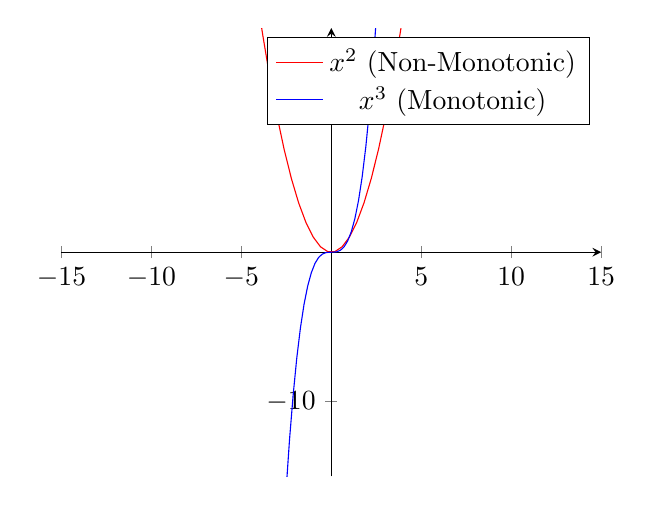
\begin{tikzpicture}
            \begin{axis}[
            axis lines = center,
            xmin = -15,
            xmax = 15,
            ymin = -15,
            ymax = 15,
            ]
                % x^2
                \addplot [
                domain=-20:20,
                samples=100,
                color=red,
                ]
                {x^2};
                \addlegendentry{$x^2$ (Non-Monotonic)}
                % x^3
                \addplot [
                domain=-10:10,
                samples=100,
                color=blue,
                ]
                {x^3};
                \addlegendentry{$x^3$ (Monotonic)}
            \end{axis}
        \end{tikzpicture}
    \end{center}

    \subsection{Even and Odd Functions}

    \textbf{Even functions} $(f(-x)=f(x))$ are unchanged when reflected across the y-axis.
    \textbf{Odd functions} $(f(-x)=-f(x)$ are unchanged when rotated $180\degree$ about the origin. \\

    \begin{center}
        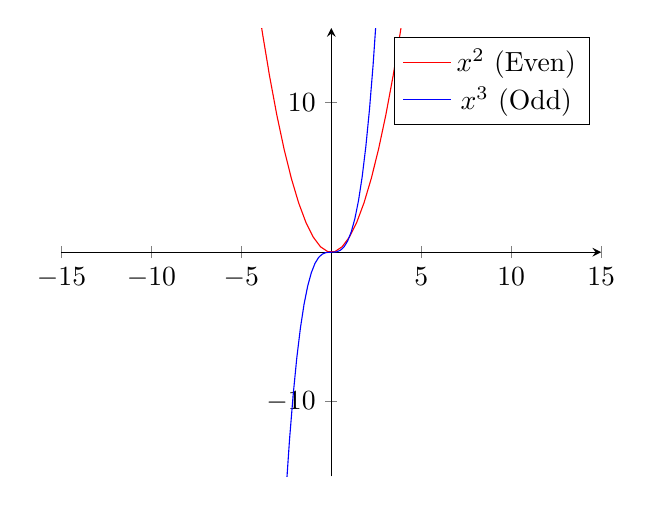
\begin{tikzpicture}
            \begin{axis}[
            axis lines = center,
            xmin = -15,
            xmax = 15,
            ymin = -15,
            ymax = 15,
            ]
                % x^2
                \addplot [
                domain=-20:20,
                samples=100,
                color=red,
                ]
                {x^2};
                \addlegendentry{$x^2$ (Even)}
                % x^3
                \addplot [
                domain=-10:10,
                samples=100,
                color=blue,
                ]
                {x^3};
                \addlegendentry{$x^3$ (Odd)}
            \end{axis}
        \end{tikzpicture}
    \end{center}

    \subsection{Piecewise and Parametric Functions}

    Functions that are defined differently across its $x$-intervals are
    \textbf{piecewise functions}. Consider the function defined below \\

    \begin{equation*}
        f(x)=
        \begin{cases}
            x^2 & ,x<2 \\
            6 & ,x=2 \\
            10-x & , 2<x\leq 6
        \end{cases}
    \end{equation*}

    \noindent The domain is then $\{x\in\mathbb{R}|x\leq 6\}$ and the graph looks like this: \\

    \begin{center}
        \begin{tikzpicture} [circ/.style={circle,draw,inner sep=2pt}]
            \begin{axis}[
            axis lines = center,
            xmin=-4.5,
            xmax=6.5,ymin=-2,
            xlabel={$x$},ylabel={$y$},
            ]
                %f(x), x < 2
                \addplot [
                red,
                smooth,
                {Stealth[bend]}-,
                domain=-4:2,
                postaction={decoration={text along path,
                text align={align=center},
                text={|\color{red}|{$y$}{${}={}$}{${x^2}$}},
                raise=-2.5ex,
                },
                decorate}]
                {x^2}
                node[pos=1,circ,fill=white]{};
                \addlegendentry{$f(x)$}
                %f(x), x = 2
                \path (2,6) node [
                circ,
                fill=red!60
                ]
                {};
                %f(x), 2 < x <= 6
                \addplot [
                red,
                samples=2,
                domain=2:6
                ]
                {10-x};
                node[pos=0,circ,fill=white]{};
                node[pos=1,circ,fill=red!60]{};
            \end{axis}
        \end{tikzpicture}
    \end{center}

    \noindent Instead of defining a single function $y=f(x)$, \textbf{Parametric Equations} are
    defined as multiple functions together, one for each variable. Hence, we can represent a
    function with $x$ and $y$ in terms of the \textbf{parameter} $t$ as below:

    \begin{center}
        \begin{tabular} {cc}
            $x=f(t)$ & $y=g(t)$
        \end{tabular}
    \end{center}

    \noindent An example of a \textbf{parametric curve}, the set of points the parameter gives
    in all the parametric equations, is the parent circle given by $x^2+y^2=r^2$. Isolating $x$
    and $y$ give our two parametric equations, $y=\pm\sqrt{r^2-x^2}$ and $x=\pm\sqrt{r^2-y^2}$. \\

    \noindent When we sketch parametric curves, we plug in values of the parameter and find
    their x and y-values, graphing each point of the form $(x,y)$ on the Cartesian Plane.
    It is important to note that parametric curves always have a \textbf{direction of motion},
    represented by arrows on the curve given by the increasing parameter $t$.

    \noindent We can \textbf{eliminate the parameter} from a set of parametric equations by
    solving for the parameter $t$ in one of the equations and plugging the value for $t$ into
    the second parametric equation.\\

    \begin{figure} [hbt!]
        \centering
        \includegraphics [scale = 0.5] {Resources/Unit9EvenMoreFunctions/param.png}
    \end{figure}

    \subsection{The Absolute Value Function}
    An \textbf{Absolute Value Function} is a function involving absolute value operations.
    The absolute value parent function is \\

    \begin{equation*}
        f(x)=|x|=
        \begin{cases}
            x, & x>0 \\
            0, & x=0 \\
            -x, & x<0
        \end{cases}
    \end{equation*}

    \noindent Absolute value functions are V-shaped and to graph them we simply choose some
    $x$-values and plot their ordered pairs. \\

    \begin{center}
        \begin{tikzpicture}
            \begin{axis}[
            axis lines = center,
            xmin = -5,
            xmax = 5,
            ymin = -5,
            ymax = 5
            ]
                % f(x)
                \addplot [
                samples=100,
                color=red,
                ]
                {abs(x)};
                \addlegendentry{$f(x)=|x|$}
            \end{axis}
        \end{tikzpicture}
    \end{center}

    \subsection{The Floor and Ceiling Functions}

    The \textbf{floor} of a number is the nearest integer down. The \textbf{ceiling} of a number
    is the nearest integer up. For 2.31, the floor is 2 and the ceiling is 3. The floor and
    ceiling of integers are the integers themselves. The floor of $x$ is represented by
    $\floor*{x}$ and the ceiling by $\ceil*{x}$. \\

    \noindent The \textbf{Floor Function} is piecewise, discontinuous at each integer, and is
    composed of the greatest integer that is less than or equal to $x$. The
    \textbf{Ceiling Function} is piecewise, discontinuous at each integer, and is composed of
    the least integer that is greater than or equal to $x$.\\

    \noindent \color{purple} \textbf{Properties of Floor and Ceiling Functions:} \color{black} \\
    1. $\floor*{x+n}=\floor*{x}+n$ for any integer $n$ \\
    2. $\floor*{x}+\floor*{-x}=\begin{cases}
                                   -1, & x \not\in \mathbb{Z}\\0, &x\in\mathbb{Z}
    \end{cases}$ \\
    3. $\floor*{x+y}=\floor*{x}+\floor*{y}=\floor*{x}+\floor*{y}+1$ \\

    \noindent Similary, all of the floor brackets can be replaced with ceiling brackets for
    their properties as well. \\

    \noindent The domain of the floor function is given by $\floor*{x}\leq x<\floor*{x}+1$. \\

    \noindent \color{blue} \textit{Example 1: Find all the values of $x$ that satisfy
    $\floor*{0.5+\floor*{x}}=20$}. \color{black} \\
    Let $y=\floor*{x}$. Then \\

    \begin{align*}
        \floor*{0.5+y} &= 20 \\
        & \iff \\
        20\leq y &+ 0.5 <21\\
        19.5\leq &y <20.5
    \end{align*}

    \noindent Since $y$ is an integer and $y=20$ is the only interval in this interval,
    this becomes $y=20=\floor*{x}$. Since any value less than 21 and greater than or equal to
    20 wil satisfy this equation, the answer is $\{x\in\mathbb{R}|20\leq x<21\}$. \\

    \begin{center}
        \begin{tikzpicture} [circ/.style={circle,draw,inner sep=1.5pt}]
            \begin{axis}[
            axis lines = center,
            xmin = -5,
            xmax = 5,
            ymin = -5,
            ymax = 5,
            xlabel={$x$},ylabel={$y$},
            ]
                %Floor function
                \addplot[red,samples=2,domain=-4:-3] {-4}
                node[pos=0,circ,fill=red!60]{}
                node[pos=1,circ,fill=white]{};
                \addplot[red,samples=2,domain=-3:-2] {-3}
                node[pos=0,circ,fill=red!60]{}
                node[pos=1,circ,fill=white]{};
                \addplot[red,samples=2,domain=-2:-1] {-2}
                node[pos=0,circ,fill=red!60]{}
                node[pos=1,circ,fill=white]{};
                \addplot[red,samples=2,domain=-1:0] {-1}
                node[pos=0,circ,fill=red!60]{}
                node[pos=1,circ,fill=white]{};
                \addplot[red,samples=2,domain=0:1] {0}
                node[pos=0,circ,fill=red!60]{}
                node[pos=1,circ,fill=white]{};
                \addplot[red,samples=2,domain=1:2] {1}
                node[pos=0,circ,fill=red!60]{}
                node[pos=1,circ,fill=white]{};
                \addplot[red,samples=2,domain=2:3] {2}
                node[pos=0,circ,fill=red!60]{}
                node[pos=1,circ,fill=white]{};
                \addplot[red,samples=2,domain=3:4] {3}
                node[pos=0,circ,fill=red!60]{}
                node[pos=1,circ,fill=white]{};
            \end{axis}
        \end{tikzpicture} \\
        \textbf{The Floor Function}
    \end{center}

    \begin{center}
        \begin{tikzpicture} [circ/.style={circle,draw,inner sep=1.5pt}]
            \begin{axis}[
            axis lines = center,
            xmin = -5,
            xmax = 5,
            ymin = -5,
            ymax = 5,
            xlabel={$x$},
            ylabel={$y$}
            ]
                %Ceiling function
                \addplot[red,samples=2,domain=-4:-3] {-4}
                node[pos=0,circ,fill=white]{}
                node[pos=1,circ,fill=red!60]{};
                \addplot[red,samples=2,domain=-3:-2] {-3}
                node[pos=0,circ,fill=white]{}
                node[pos=1,circ,fill=red!60]{};
                \addplot[red,samples=2,domain=-2:-1] {-2}
                node[pos=0,circ,fill=white]{}
                node[pos=1,circ,fill=red!60]{};
                \addplot[red,samples=2,domain=-1:0] {-1}
                node[pos=0,circ,fill=white]{}
                node[pos=1,circ,fill=red!60]{};
                \addplot[red,samples=2,domain=0:1] {0}
                node[pos=0,circ,fill=white]{}
                node[pos=1,circ,fill=red!60]{};
                \addplot[red,samples=2,domain=1:2] {1}
                node[pos=0,circ,fill=white]{}
                node[pos=1,circ,fill=red!60]{};
                \addplot[red,samples=2,domain=2:3] {2}
                node[pos=0,circ,fill=white]{}
                node[pos=1,circ,fill=red!60]{};
                \addplot[red,samples=2,domain=3:4] {3}
                node[pos=0,circ,fill=white]{}
                node[pos=1,circ,fill=red!60]{};
            \end{axis}
        \end{tikzpicture} \\
        \textbf{The Ceiling Function}
    \end{center}

    \subsection{The Fractional Part Function}

    The \textbf{Fractional Part Function} is defined as $f(x)=\{x\}=x-\floor*{x}$.
    For nonnegative real numbers, the fractional part is simply the part after the decimal.
    For example, $\{3.64\}=3.64-\floor*{3.64}=3.64-3=0.64$. \\

    \noindent \textbf{Properties of the Fractional Part Function:} \\
    1. $0\leq\{x\}<1$ and $0=\{x\}$ if and only if $x$ is an integer \\
    2. $\{x\}+\{-x\}=$

    \begin{cases}
        0 & \text{if } x \text{ is an integer} \\
        1 & \text{otherwise}
    \end{cases}

    \noindent 3. If $a$ and $b$ are integers and $b>0$ then $\{\frac{a}{b}\}=\frac{r}{b}$, where
    $r$ is the remainder from dividing $a$ by $b$.

    \begin{center}
        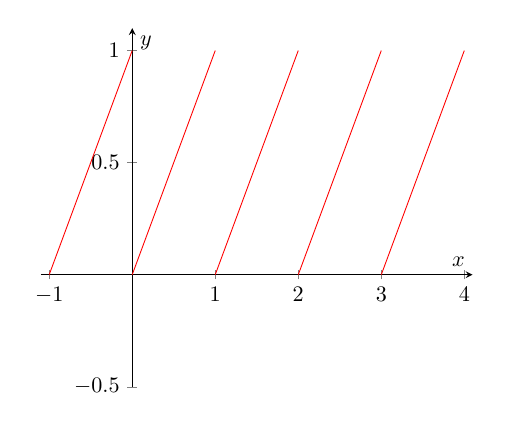
\begin{tikzpicture}[circ/.style={circle,draw,inner sep=1.5pt}, scale = 0.8]
            \begin{axis}[
            axis lines = center,
            xmin = -1.1,
            xmax = 4.1,
            ymin = -0.5,
            ymax = 1.1,
            xlabel={$x$},
            ylabel={$y$}
            ]
                %Coordinates
                \coordinate (A) at (-1,0);
                \coordinate (B) at (0,1);
                \coordinate (C) at (0,0);
                \coordinate (D) at (1,1);
                \coordinate (E) at (1,0);
                \coordinate (F) at (2,1);
                \coordinate (G) at (2,0);
                \coordinate (H) at (3,1);
                \coordinate (I) at (3,0);
                \coordinate (J) at (4,1);
                %%%
                %Functions
                \draw[color=red] (A) -- (B);
                \draw[color=red] (C) -- (D);
                \draw[color=red] (E) -- (F);
                \draw[color=red] (G) -- (H);
                \draw[color=red] (I) -- (J);
                %%%
            \end{axis}
        \end{tikzpicture} \\
        \textbf{The Fractional Part Function}
    \end{center}

    \pagebreak
%%%-------------------------------------------NEW SECTION--------------------------------------%%%


    \section{Conics}

    \subsection{Introduction to Conics}

    From Analytic Geometry, \textbf{Conic Sections} are the intersection of a plane and
    2 opposite-facing solid cones from different angles. \\

    \begin{figure} [hbt!]
        \centering
        \includegraphics [scale=0.6] {Resources/Unit10Conics/conics.PNG}
    \end{figure}

    \noindent These curves can be defined using a straight line (\textbf{directrix}) and a
    point (\textbf{focus}). The distance from the focus to a point on the curve and the
    distance perpendicularly from the directrix to that point will always be the same ratio.
    For ellipses, this ratio is less than 1. For parabolas, the ratio is 1, hence the
    distances are equal. For hyperbolas, this ratio is greater than 1. This ratio is called
    \textbf{eccentricity}, which graphically shows us how "un-circular" the curve is. The
    larger the eccentricity, the less curved it is. Circles have an eccentricity of 0. \\

    \begin{figure} [hbt!]
        \centering
        \includegraphics [scale=0.5] {Resources/Unit10Conics/ecc.PNG}
    \end{figure}

    \noindent The \textbf{latus rectum} runs parallel to the directrix and passes through the focus. \\
    \noindent \textbf{Length of the Latus Rectum:} \\

    \begin{center}
        \begin{tabular}{|c|c|}
            \hline
            \textbf{Parabolas} & 4x focal length  \\
            \hline
            \textbf{Circles}   & the diameter     \\
            \hline
            \textbf{Ellipses}  & $\frac{2b^2}{a}$ \\
            \hline
        \end{tabular}
    \end{center}

    \noindent Above, $a$ and $b$ are the \textbf{major} and \textbf{minor axes}, respectively.

    \begin{figure} [hbt!]
        \centering
        \includegraphics[scale = 0.6] {Resources/Unit10Conics/latrect.PNG}
        \includegraphics[scale = 0.6] {Resources/Unit10Conics/lactrect2.PNG}
    \end{figure}

    \noindent The \textbf{General Equation} that covers all conic equations is given by \\

    \begin{equation*}
        Ax^2+Bxy+Cy^2+Dx+Ey+F=0
    \end{equation*}

    \noindent where $A,B,C,D,E,F$ are all constants. \\

    \noindent \color{purple} \textbf{Process to Determine Conic Type from General Form:} \color{black} \\
    1. Are both variables squared? \\
    If no, it's a parabola. If yes, go to next step. \\
    2. Do the squared terms have opposite signs? \\
    If yes, it's a hyperbola. If no, go to next step. \\
    3. Are the squared terms multiplied by the same number? \\
    If yes, it's a circle. If no, it's an ellipse.

    \pagebreak

    \subsection{Ellipses}
    For the equations below, $a$ is the length of half of the major axis, $b$ is the length of
    half of the minor axis, and $A,C,D,E,F$ are constants, respectively. \\

    \begin{center}
        \begin{tabular}{|c|c|}
            \hline
            \textbf{General Form}
            & $Ax^2+Cy^2+Dx+Ey+F=0$                       \\
            \hline
            \textbf{Standard Form, Horizontal Major Axis}
            & $\frac{(x-h)^2}{a^2}+\frac{(y-k)^2}{b^2}=1$ \\
            \hline
            \textbf{Standard Form, Vertical Major Axis}
            & $\frac{(x-h)^2}{b^2}+\frac{(y-k)^2}{a^2}=1$ \\
            \hline
        \end{tabular}
    \end{center}

    \noindent Center: $(h,k)$ \\
    Length of Major Axis: $2a$ \\
    Length of Minor Axis: $2b$ \\
    Distance between center and foci, represented by $c$, is $c^2=a^2-b^2,a>b>0$ \\

    \noindent The major axis runs between the vertices, whereas the minor axis runs between
    the co-vertices. \\

    \begin{figure} [hbt!]
        \centering
        \includegraphics [scale=0.6] {Resources/Unit10Conics/ellipse1.jpg}
    \end{figure}

    \noindent \color{purple} \textbf{Graphing Ellipses:} \color{black} \\
    Determine the major axis, vertices, co-vertices, and foci. \\
    \textbf{Equation is in form $\frac{(x-h)^2}{a^2}+\frac{(y-k)^2}{b^2}=1, a>b$}

    \begin{center}
        \begin{tabular} {|c|c|}
            \hline
            Center                         & $(h,k)$              \\
            \hline
            Major Axis                     & parallel to $x$-axis \\
            \hline
            Coordinates of the Vertices    & $(h\pm a, k)$        \\
            \hline
            Coordinates of the Co-vertices & $(h,k \pm b)$        \\
            \hline
            Coordinates of the Foci        & $(h\pm c, k)$        \\
            \hline
        \end{tabular}
    \end{center}

    \noindent \textbf{Equation is in form $\frac{(x-h)^2}{b^2}+\frac{(y-k)^2}{a^2}=1, a>b$} \\

    \begin{center}
        \begin{tabular} {|c|c|}
            \hline
            Center                         & $(h,k)$              \\
            \hline
            Major Axis                     & parallel to $y$-axis \\
            \hline
            Coordinates of the Vertices    & $(h, k\pm a)$        \\
            \hline
            Coordinates of the Co-vertices & $(h\pm b, k)$        \\
            \hline
            Coordinates of the Foci        & $(h, k\pm c)$        \\
            \hline
        \end{tabular}
    \end{center}

    \noindent \color{blue} \textit{Example 1: Graph $\frac{(x+2)^2}{4}+\frac{(y-5)^2}{9}=1$}
    \color{black} \\
    \noindent Because $a$ is the always the bigger number, $a^2=9$ and $b^2=4$. Because
    $9>4$ the major axis is parallel to the $y$-axis. The center $(h,k)$ is then $(-2,5)$. The
    vertices are $(h,k\pm a)=(-2,2),(-2,8)$. The co-vertices are $(h\pm b,k)=(-4,5),(0,5)$.
    Since $c^2=a^2-b^2=9-4=5\implies c=\pm\sqrt{5}$, the foci are $(h,k\pm c)=(-2,5-\sqrt{5}),
    (-2,5\pm 5)$. \\

    \begin{figure} [hbt!]
        \centering
        \includegraphics [scale=0.5] {Resources/Unit10Conics/ellipse2.PNG}
    \end{figure}

    \noindent \color{blue} \textit{Example 2: Graph the ellipse given by
    $4x^2+9y^2-40x+36y+100=0$} \color{black}  \\

    \begin{align*}
        (4x^2-40x)+(9y^2+36y) &= -100 \\
        4(x^2-10x) + 9(y^2+4y) &= -100 \\
        4(x^2-10x+25)+9(y^2+4y+4) &= -100 + 100 +36 \\
        4(x-5)^2+9(y+2)^2 &= 36 \\
        \frac{(x-5)^2}{9}+\frac{(y+2)^2}{4}=1
    \end{align*}

    \noindent Because $9>4$. the major axis is parallel to the $x$-axis. Since $a^2=9$ and
    $b^2=4$, $c^2=9-4\implies c=\pm \sqrt{5}$. The center is $(5, -2)$. The vertices are
    $(2,-2),(8,-2)$. The co-vertices are $(5,-4),(5,0)$. The foci are $(5-\sqrt{5},-2),
    (5+\sqrt{5},-2)$. \\

    \begin{figure} [hbt!]
        \centering
        \includegraphics [scale=0.5] {Resources/Unit10Conics/ellipse3.PNG}
    \end{figure}

    \subsection{Circles}
    A \textbf{circle} is the set of all points on a plane that are a fixed distance from the
    center. A circle is not a function because it fails the vertical line test. A circle is a
    special type of ellipse with equations below. \\

    \begin{center}
        \begin{tabular} {|c|c|}
            \hline
            \textbf{General Form}
            & $x^2+y^2+Cx+Dy+E=0$   \\
            \hline
            \textbf{Standard Form}
            & $(x-h)^2+(y-k)^2=r^2$ \\
            \hline
        \end{tabular}
    \end{center}

    \noindent Above, the center is given by $(h,k)$ and the radius as $r$.

    \noindent \color{purple} \textbf{Graphing Circles:} \color{black} \\
    Determine the center $(h,k)$ and radius $r$ and graph it.

    \subsection{Parabolas}
    We have already graphed and worked with parabolas in the past, so here are the general
    forms of parabolas when used in the context of conics. \\

    \begin{center}
        \begin{tabular} {|c|c|c|}
            \hline
            \textbf{Parabola, Horizontal Axis}
            & $(y-k)^2=4p(x-h),p\not=0$
            & Vertex is $(h,k)$ \\
            & & Focus is $(h+p,k)$            \\
            & & Directrix is the line $x=h-p$ \\
            & & Axis is the line $y=k$        \\
            \hline
            \textbf{Parabola, Vertical Axis}
            & $(x-h)^2=4p(y-k),p\not=0$
            & Vertex is $(h,k)$ \\
            & & Focus is $(h,k+p)$            \\
            & & Directrix is the line $y=k-p$ \\
            & & Axis is the line $x=h$        \\
            \hline
        \end{tabular}
    \end{center}

    \subsection{Hyperbolas}
    Hyperbolas look like this: \\
    \begin{figure} [hbt!]
        \centering
        \includegraphics [scale=0.3] {Resources/Unit10Conics/hyperbola.png}
    \end{figure}

    \begin{center}
        \begin{tabular} {|c|c|}
            \hline
            \textbf{General Form}
            & $Ax^2-Cy^2+Dx+Ey+F=0$                       \\
            \hline
            \textbf{Hyperbola, Horizontal Transverse Axis}
            & $\frac{(x-h)^2}{a^2}-\frac{(y-k)^2}{b^2}=1$ \\
            \hline
            \textbf{Hyperbola, Vertical Transverse Axis}
            & $\frac{(y-k)^2}{a^2}-\frac{(x-h)^2}{b^2}=1$ \\
            \hline
        \end{tabular}
    \end{center}

    \noindent Center: $(h,k)$ \\
    Distance between vertices: $2a$ \\
    Distance between foci: $2c$ \\
    $c^2=a^2+b^2$ \\

    \noindent The eccentricity, $e$, has the formula \\
    $e=\frac{\sqrt{a^2+b^2}}{a}$  \\

    \noindent The reciprocal function $f(x)=\frac{1}{x}$ is a hyperbola.

    \pagebreak
%%%-------------------------------------------NEW SECTION--------------------------------------%%%


    \section{Sequences and Series}

    \subsection{Introduction to Sequences and Series}
    A \textbf{sequence} is an ordered list of numbers, whereas a \textbf{series} is the
    sum of the terms of a sequence. We can represent a series with $\{a_n\}^\infty_{n=1}$,
    where the sequence starts with index $n=1$ and runs to infinity. The other notation,
    summation notation, is written $\sum^{10}_{n=1}a_n$, where the sequence runs from $n=1$
    to infinity. \\

    \noindent For example, the expansion of
    $\{a_n\}_{n=1}^{n=10}$ is $a_n=n^2=1,4,,9,16,25,36,49,64,81,100$. \\

    \noindent Conventionally, the following symbols are used:

    \begin{center}
        \begin{tabular} {|c|c|}
            \hline
            $a$
            & first term in sequence                                                    \\
            \hline
            $n$
            & number of terms in sequence                                               \\
            \hline
            $S_n$
            & sum of first $n$ terms in sequence                                        \\
            \hline
            $d$
            & Common difference between any two consecutive terms, arithmetic sequences \\
            \hline
            $r$
            & Common ratio between two consecutive terms, geometric sequences           \\
            \hline
        \end{tabular}
    \end{center}

    \subsection{Arithmetic Progressions} \\
    \textbf{Arithmetic Progressions} are sequences containing numbers which differ from each
    other by a common difference, $d$. \\

    \noindent \textbf{Formula for Arithmetic Sequences} \\

    \begin{equation*}
        a_n=a_1+d(n-1)
    \end{equation*}

    \noindent $a_n$ is the $n^{th}$ term, $a_1$ is the first term, $n$ is the index \\

    \noindent  The sum of the first $n$ terms is given by one of the three formulas. \\

    \begin{align*}
        S_n=\frac{n}{2}[2a+d(n-1)] \\
        S_n=\frac{n}{2}[a+a_n] \\
        S_n=n\cdot (middle term)
    \end{align*}

    \noindent Find the sum of the first 50 odd positive integers. \\

    \begin{equation*}
        S_n=\frac{n}{2}(2a+d(n-1))
        \implies
        S_{50}=25\cdot (2+49\cdot 2)=2500
    \end{equation*}

    \subsection{Geometric Sequences and Series}
    \textbf{Geometric Sequences} include terms that are multiplied by a ratio iteratively.
    They are given by the following formula. \\

    \begin{equation*}
        a_n=a\cdot r^{n-1}
    \end{equation*}

    \noindent $a_n$ is the $n^{th}$ term, $a$ is the first term, $r$ is the common ratio. \\

    \noindent The sum of a geometric sequence is given by \\

    \begin{equation*}
        S_n = \begin{cases}
                  a\cdot (\frac{r^n-1}{r-1}), & r\not=1 \\
                  a\cdot n, & r=1
        \end{cases}
    \end{equation*}

    \noindent The sum to infinity of a geometric sequence, where $|r|<1$, is given by \\

    \begin{equation*}
        S_\infty=\frac{a}{1-r}
    \end{equation*}

    \noindent \color{blue} \textit{Example: After striking the floor, a tennis ball bounces
    to $\frac{2}{3}$ of the height from which it last fell. What is the total vertical
    distance it travels before it comes to rest when it is dropped from a vertical height of
    100$m$?} \color{black} \\

    \noindent If $h$ is the height in meters, $e$ is a number such that $0<e<1$, and $S$ is
    the total vertical distance covered before coming to rest, then \\

    \begin{align*}
        S &= h+2(eh)+2(e^2h)+2(e^3h)+2(e^4)h + \dots \\
        &= h+2eh(1+e+e^2+e^3+\dots) \\
        &= h+2eh \cdots \frac{1}{1-e}, \because e<1 \\
        &= h\left(\frac{1+e}{1-e}\right)
    \end{align*}

    \noindent Since it is given that $h=100$ and $e=\frac{2}{3}$, \\

    \begin{equation*}
        S=100\left(\frac{1+\frac{2}{3}}{1-\frac{2}{3}}\right)=500 \text{ meters}
    \end{equation*}

    \subsection{Binomial Expansion}
    The \textbf{Binomial Theorem} allows us to expand binomials such that \\

    \begin{equation*}
        (a+b)^n
        = \sum^n_{k=0}\binom{n}{k}a^{n-k}b^k
    \end{equation*}

    \noindent where $\binom{n}{k}$, pronounced "n choose k" because it describes how many
    ways to choose $k$ elements from a set of $n$, is given by the formula \\

    \begin{equation*}
        \binom{n}{k}=\frac{n!}{k!(n-k)!}
    \end{equation*}

    \noindent In the Binomial Theorem, $\binom{n}{k}$ determines the coefficients of the
    expanded binomial. Coefficients of Binomials follow Pascal's Triangle and they match up
    like so: \\

    \begin{figure} [hbt!]
        \centering
        \includegraphics[scale = 0.5] {Resources/Unit11Sequences/pascal.PNG}
    \end{figure}

    \noindent \color{blue} \textit{Example 1: Expand $(y+5)^4$} \color{black} \\

    \begin{align*}
        (y+5)^4 &= \binom{4}{0}y^45^0
        + \binom{4}{1}y^35^1
        + \binom{4}{2}y^25^2
        + \binom{4}{3}y^15^3
        + \binom{4}{4}y^05^4 \\
        &= y^4+20y^3+150y^2+500y+625
    \end{align*}

    \noindent \color{blue} \textit{Example 2: What is the coefficient of $x^3 in (2x+4)^8?$}
    \color{black} \\
    The term containing $x^3$ is \\

    \begin{align}
        \binom{8}{5}(2x)^34^5 &= 56(2x^3)(4^5) \\
        &= 458752x^3
    \end{align}

    \noindent Hence, the coefficient is 458752.

    \pagebreak
%%%%---------------------------------------------NEW SECTION------------------------------------------


    \section{The Cauchy-Schwartz Inequality}

    The Cauchy-Schwartz Inequality, or the Cauchy-Bunyakovsky-Schwartz Inequality, states
    that for all sequences of real numbers $a_i$ and $b_i$, we have \\

    \begin{equation*}
        (\sum^n_{i=1}a_i^2)
        (\sum^n_{i=1}b_i^2)
        \geq
        (\sum^n_{i=1}a_ib_i)^2
    \end{equation*}

    \noindent Equality holds if and only if $a_i=kb_i$ for some non-zero constant
    $k\in\mathbb{R}$. \\

    \noindent \color{blue} \textit{Example: If $x^2+y^2+z^2=1$, what is the maximum
    value of $x+2y+3z$?} \color{black} \\

    \noindent We have $(x+2y+3z)^2\leq(1^2+2^2+3^2)(x^2+y^2+z^2)=14$. Hence, $x+2y+3z\leq\sqrt{14}$
    with equality holding when $\frac{x}{1}=\frac{y}{2}=\frac{z}{3}$. Together with
    $x^2+y^2+z^2=1$, we get \\

    \begin{equation*}
        x=\frac{1}{\sqrt{14}},
        y=\frac{2}{\sqrt{14}},
        z=\frac{3}{\sqrt{14}}
    \end{equation*}

    \pagebreak
%%%%---------------------------------------------NEW SECTION------------------------------------------


    \section{Symbolic Logic and Proofs}

    \subsection{Statements and Logical Operators}
    A \textbf{proof} is an argument from \textbf{hypotheses} to a \textbf{conclusion}.
    Proofs usually begin with \textbf{premises}, statements that are known to be true.
    The \textbf{Rule of Premises} says that you may write down a premise at any point in a
    proof. The rule of \textbf{modus ponendo ponens} says that if you know $P$ and
    $P\rightarrow Q$, you can write down $Q$. \\

    \noindent Mathematical statements can only be true or false. The letters $p$ and $q$
    often denote statements. \\

    \noindent \color{purple} \textbf{Logical Operators:} \color{black} \\
    \textbf{Not ($\neg$)}: The statement "not $p$" is called the \textbf{negation} of $p$. \\

    \begin{center}
        \begin{tabular} {|c|c|}
            \hline
            $p$ & $\neg p$ \\
            \hline
            0   & 1        \\
            \hline
            1   & 0        \\
            \hline
        \end{tabular}
    \end{center}

    \noindent \textbf{Double Negation} states that $\neg\neg P$ is logically equivalent to $P$.

    \noindent \textbf{And (\&)}: \\

    \begin{center}
        \begin{tabular} {|c|c|c|}
            \hline
            $p$ & $q$ & $p\& q$ \\
            \hline
            1 & 1 & 1 \\
            \hline
            1 & 0 & 0 \\
            \hline
            0 & 1 & 0 \\
            \hline
            0 & 0 & 0 \\
            \hline
        \end{tabular}
    \end{center}

    \noindent \textbf{Or: ($\vert\vert$)} \\

    \begin{center}
        \begin{tabular} {|c|c|c|}
            \hline
            $p$ & $q$ & $p||q$ \\
            \hline
            1   & 1   & 1      \\
            \hline
            1   & 0   & 1      \\
            \hline
            0   & 1   & 1      \\
            \hline
            0   & 0   & 0      \\
            \hline
        \end{tabular}
    \end{center}

    \noindent\textbf{If\dots then ($\rightarrow)$:} \\

    \begin{center}
        \begin{tabular} {|c|c|c|}
            \hline
            $p$ & $q$ & $p\rightarrow q$ \\
            \hline
            1   & 1   & 1                \\
            \hline
            1   & 0   & 0                \\
            \hline
            0   & 1   & 1                \\
            \hline
            0   & 0   & 1                \\
            \hline
        \end{tabular}
    \end{center}

    \noindent If $p$ is false then $p\rightarrow q$ is \textbf{vacuously true}.
    For example, the statement all cell phones in the room are turned off is true even
    if there are no cell phones in the room. \\

    \noindent \textbf{If and only if ($\iff$):} \\

    \begin{center}
        \begin{tabular} {|c|c|c|}
            \hline
            1 & 1 & 1 \\
            \hline
            1 & 0 & 0 \\
            \hline
            0 & 1 & 0 \\
            \hline
            0 & 0 & 1 \\
            \hline
        \end{tabular}
    \end{center}

    \noindent When $p\iff q$ is true, $p$ and $q$ are \textbf{equivalent}. \\

    \noindent \textbf{Quantifiers} include the phrases "for every ($\forall$)" and
    "there exists (\exists)". $Consider the sentence "$x$ is even". This does not count
    as a statement since we can't say whether or not it is true or false since we don't
    know what $x$ is. We can make this a statement by saying "an integer $x$ is even if
    there exists an integer $y$ such that $x=2y$".$

    \subsection{Proof Methods}
    \noindent \color{purple} \textbf{Proof by Cases:} \color{black} \\
    \color{blue} \textit{Example: For every integer $x$, the integer $x(x+1)$ is even.} \color{black}  \\
    Let $x$ be any integer. Then $x$ is even or odd. \\
    Case 1: suppose $x$ is even. Choose an integer $k$ such that $x=2k$. Then $x(x+1)=2k(2k+1)$.
    Let $y=k(2k+1)$; then $y$ is an integer and $x(x+1)=2y$ so $x(x+1)$ is even. \\
    Case 2: suppose $x$ is odd. Choose an integer $k$ such that $x=2k+1$. Then
    $x(x+1)=(2k+1)(2k+2)$. Let $y=(2k+1)(k+1)$; then $x(x+1)=2y$, so $x(x+1)$ is even.
    $\blacksquare$ \\

    \noindent \color{purple} \textbf{Proof by Contradiction:} \color{black} \\
    Suppose we want to prove that statement $p$ is true. We begin by assuming $p$ is false.
    We then deduce a \textbf{contradiction} (some statement about $q$ we know to be false).
    If we succeed, then our assumption that $p$ is false must be wrong. Hence $p$ would have
    to be true.

\end{document}